\section{File-level content addressable storage models}
\label{sec:file_adressable}


\subsection{Benefit of file-level content addressable storage}


\subsection{Two models -- Layer recompression model and layer reconstruction model}

\begin{figure}
	\centering
	%\includegraphics [width=0.45\textwidth]{plots/exp-total-stev-erase.eps}
	\subfigure[Recompression layers]{\label{fig:per_layer_ratio_fcnt_cdf}
		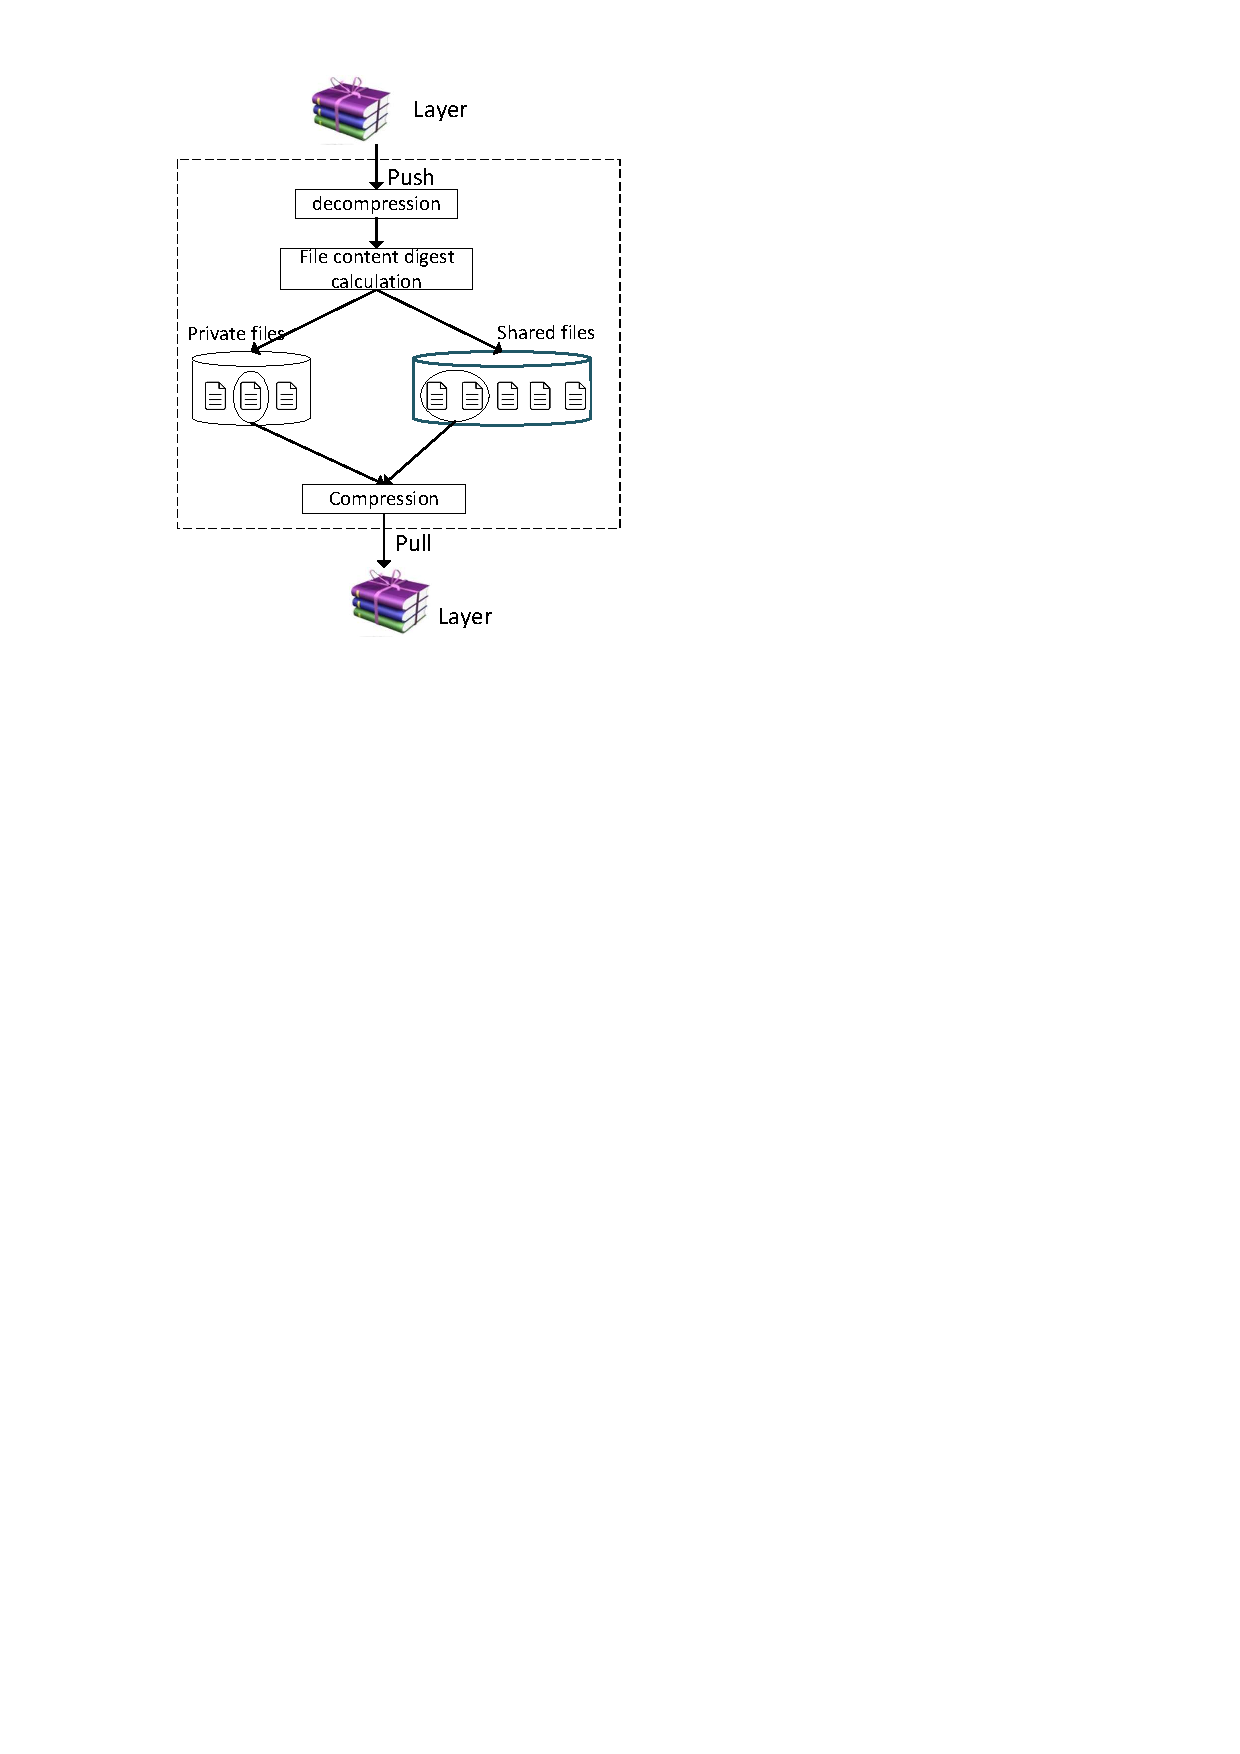
\includegraphics [width=0.21\textwidth]{graphs/graph_compression_layers.pdf}
	}
	\subfigure[Reconstruct layers]{\label{fig:per_layer_ratio_fcnt_pdf}
		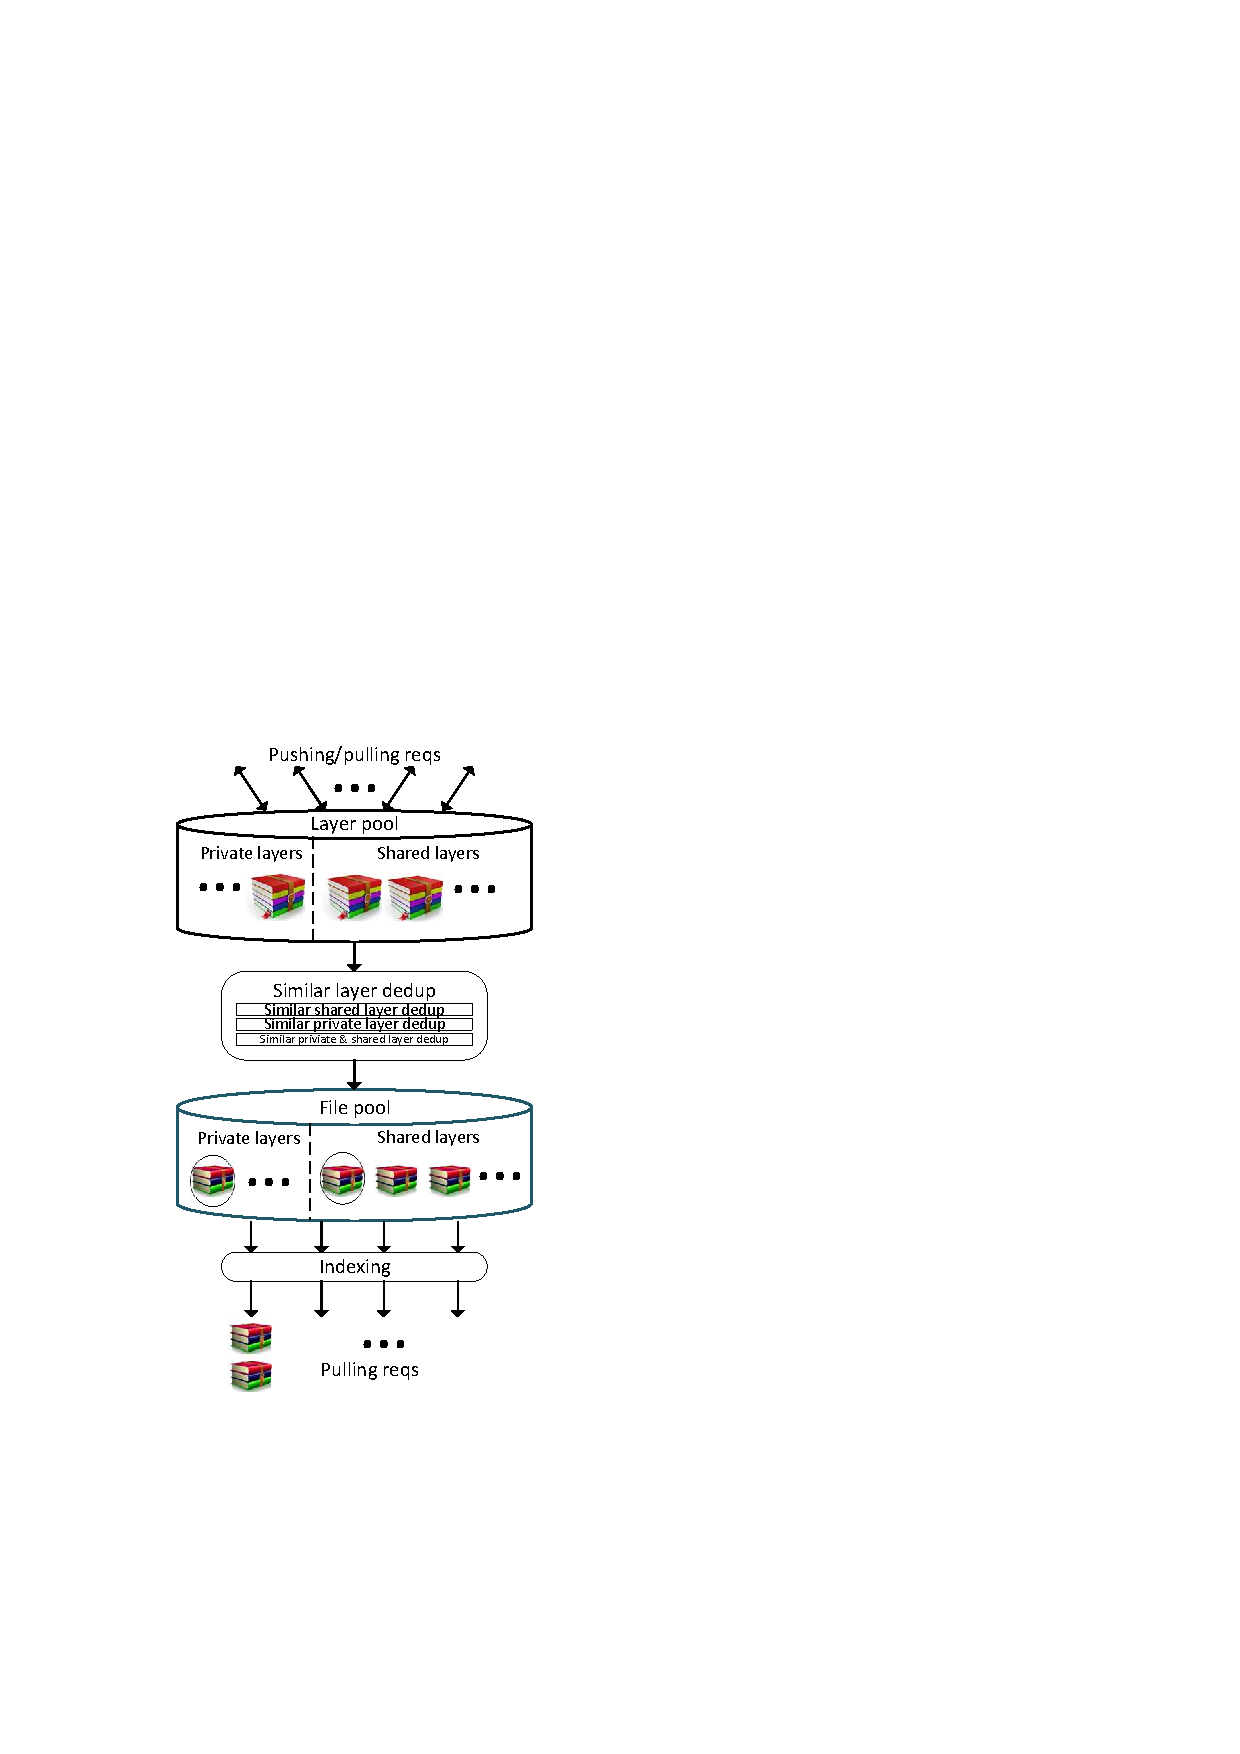
\includegraphics [width=0.24\textwidth]{graphs/graph_reconstruct_layers.pdf}
	}
	\caption{File-level content addressable storage model}
	\label{fig:eval-stdev-erasure-cnt}
\end{figure}

\subsection{Performance overhead discussion for layer recompression model}

\subsubsection{Recompression overhead} Compression time. Other are negligible. 

\subsubsection{Trade-offs between dedup ratio and recompression overhead}

\paragraph{Dedup ratio VS. performance overhead}

\subsection{Performance overhead discussion for layer reconstruction model}

\subsubsection{Reconstruction overhead}

\paragraph{Smaller than recompression model} the registry can prepare the reconstructed layers before users issue a pull request. But this model requires users to rebuild two layers.

\subsubsection{Trade-offs between dedup ratio and reconstruction overhead}

\paragraph{Dedup ratio VS. Rebuild overhead}

\subsection{Evaluation results}